\documentclass[12pt, a4paper]{article}
\usepackage{exercise}
\usepackage{amsmath}
\usepackage{amsfonts}
\usepackage{siunitx}
\usepackage[shortlabels]{enumitem}
\usepackage[margin=2.5cm]{geometry}
\usepackage[french]{babel}
\usepackage{graphicx}
\usepackage[justification=centering]{caption}
\usepackage{array}
\usepackage{lmodern}
\usepackage[upright]{fourier}
%\usepackage{showframe}

\graphicspath{ {./rsc/} }
% New definition of square root:
% it renames \sqrt as \oldsqrt
\let\oldsqrt\sqrt
% it defines the new \sqrt in terms of the old one
\def\sqrt{\mathpalette\DHLhksqrt}
\def\DHLhksqrt#1#2{%
\setbox0=\hbox{$#1\oldsqrt{#2\,}$}\dimen0=\ht0
\advance\dimen0-0.2\ht0
\setbox2=\hbox{\vrule height\ht0 depth -\dimen0}%
{\box0\lower0.64pt\box2}}

\sisetup{inter-unit-product=\ensuremath{{}\cdot{}}}

\renewcommand{\ExerciseHeader}
{
  \par\noindent
  \textbf{\large \ExerciseName\ \ExerciseHeaderNB\ExerciseHeaderTitle\ExerciseHeaderOrigin}%
  \par\nopagebreak\medskip
}

\newenvironment{conditions}
  {\par\vspace{\abovedisplayskip}\noindent\begin{tabular}{>{$}l<{$} @{${\quad}={\quad}$} l}}
  {\end{tabular}\par\vspace{\belowdisplayskip}}

\renewcommand{\ExerciseName}{Exercice}

\def\arraystretch{1.5}

\begin{document}
    
    \title{Exercices du Chapitre des Ondes Mécaniques \\ \Large{Pages 310-312}}
    \author{Diego Van Overberghe}
    \date{9 Mai 2020}
    \maketitle

    \begin{Exercise}[number={24}]
        \begin{enumerate}[1.]
            \item Une onde mécanique est la propagation d'une perturbation dans un milieu materiel. Elle est mécanique parce que elle agit en deplaçant la matière.
        \item   \begin{equation*}
                    v_{exp}=\frac{d}{\Delta T}
                    \iff v_\text{exp}=\frac{9\ 549{,}9\times 1{,}949}{54{,}6}
                    \iff v_\text{exp}=3{,}41\times 10^2\ \si{m.s^{-1}}
                \end{equation*} où
                \begin{conditions}
                    v_{exp}  & La célérité de l'onde (en $\si{m.s^{-1}}$) \\
                    d        & La distance (en $\si{m}$) \\
                    \Delta T & Différence de temps (en $\si{s}$)
                \end{conditions}

        \item D'après le texte, la célérité du son dépend \textit{a priori} de la température ambiente.                
        \end{enumerate}
    \end{Exercise}

    \begin{Exercise}[number={25}]
        \begin{enumerate}[1.]
            \item On peut mesurer le retard de l'arrivée du son à chaque microphone.
            \item   \begin{enumerate}[a.]
                        \item   \begin{equation*}
                                    v=\frac{M_1M_2}{\Delta T}
                                    \iff v=\frac{2{,}00}{0{,}006}
                                    \iff v=3{,}33\times 10^2\ \si{m.s^{-1}}
                                \end{equation*}
                                \begin{equation*}
                                    v=\frac{M_2M_3}{\Delta T}
                                    \iff v=\frac{3{,}00}{0{,}009}
                                    \iff v=3{,}33\times 10^2\ \si{m.s^{-1}}
                                \end{equation*}
                        \item Oui, les résultats sont cohérents. C'est à peu pres 340 $\si{m.s^{-1}}$
                    \end{enumerate}
        \end{enumerate}
    \end{Exercise}

    \begin{Exercise}[number={27}]
        \begin{enumerate}[1.]
            \item L'onde ultrason est mécanique parce qu'elle est la propagation d'une perturbation dans un milieu materiel. L'onde est progressive parce qu'il s'agit de slaves et non une emission continuelle.
            \item   \begin{enumerate}[a.]
                        \item L'emetteur est le {A}, le récepteur est le {B}, c'est dit dans la consigne.
                        \item Le retard est de à peu pres $2{,}0\ \si{ms}$.
                    \end{enumerate}
            \item   \begin{enumerate}[a.]
                        \item   \begin{equation*}
                                    v=\frac{d}{\Delta T}
                                    \iff d=v\times\Delta T
                                    \iff d=340\times 2{,}0\times 10^{-3}
                                    \iff d=6{,}80\times 10^{-1}\ \si{m}
                                \end{equation*}
                                La distance qui sépare l'emetteur et le récepteur est donc $3{,}40\times 10^{-1}\ \si{m}$.
                        \item On peut donc utiliser les ultrasons pour faire l'écholocalisation.
                    \end{enumerate}
        \end{enumerate}
    \end{Exercise}

    \begin{Exercise}[number={28}]
        \begin{itemize}
            \item[] Aprés un déplacement de valeur $D$, les ondes sont en phase. Ceci revient à dire que la longeur d'onde $D=n\lambda$. L'énoncé explique que les ondes ont été en phase cinq fois, donc $n=5$. On calcule aussi la période $T=\frac{7}{3}\ \si{ms}$.
            \begin{equation*}
                v=\frac{5\lambda}{5T}
                \iff v=\frac{3{,}85}{5\times\frac{7}{3}\times 10^{-3}}
                \iff v=3{,}3\times 10\ \si{m.s^{-1}} \pm 0{,}1\ \si{m.s^{-1}}
            \end{equation*} où
            \begin{conditions}
                v & Célérité (en $\si{m.s^{-1}}$) \\ 
                \lambda & Longeur d'Onde (en $\si{m}$) \\
                T & Période (en $\si{s}$) 
            \end{conditions}
        \end{itemize}
    \end{Exercise}

    \begin{Exercise}[number={30}]
        \begin{enumerate}[1.]
            \item   \begin{enumerate}[a.]
                        \item La longeur d'onde est la longeur qui sépare le début et le fin d'un motif périodique.
                        \item La longeur d'onde peut etre calculée en divisant une distance par le nombre de fois que le motif à pris lieu dans cette distance.
                        \item $6\ \si{cm}$ sur le déssin corréspond à $2{,}7\ \si{cm}$ en réalité. On mesure que en $2{,}0\ \si{cm}$ en sur le déssin, le motif s'est répété quatre fois. C'est-à-dire que en réalité, en $4{,}4\ \si{cm}$, le motif se répète quatre fois. On calcule donc, $\lambda=1{,}1\ \si{cm}$.
                    \end{enumerate}
            \item \ \\\parbox{\linewidth}{
                        \centering
                        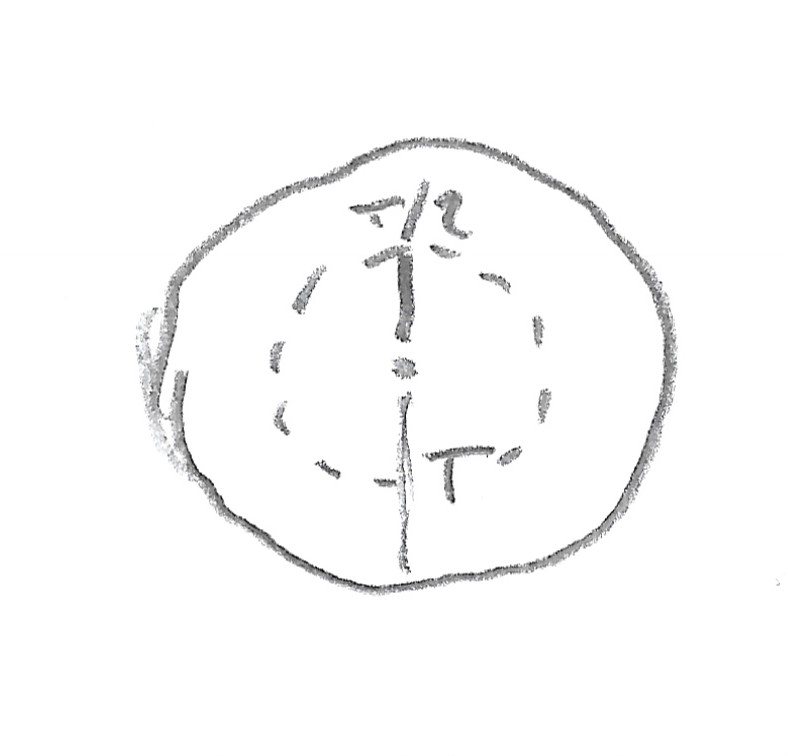
\includegraphics[width=5cm]{EX30img1.jpg}
                        \captionof{figure}{Représentation de l'allure de la surface de l'eau, où le trait solide représente l'onde à l'instant $t+T$, et les pointillés l'onde à l'instant $t+\frac{T}{2}$}
                    } \bigbreak
        \end{enumerate}
    \end{Exercise}

    \begin{Exercise}[number={32}]
        \begin{enumerate}[1.]
            \item   \begin{enumerate}[a.]
                \item $1{,}1\ \si{cm}$ sur le dessin corréspond à $3\ \si{cm}$ en réalité. \\ $2\lambda_\text{avant}=3\ \si{cm} \iff \lambda_\text{avant}=1{,}5\ \si{cm}$
                \item $4\lambda_\text{après}=3\ \si{cm} \iff \lambda_\text{après}=0{,}8\ \si{cm}$
            \end{enumerate}
            \item Il paraît que lors de la diffraction, la longeur d'onde est divisée en deux.
            \item On ne connaît pas la période. Il est possible que la célérité augemente, reste constante, ou diminue.
        \end{enumerate}
    \end{Exercise}
\end{document}